\documentclass[11pt,a4paper,]{article}
\usepackage{lmodern}

\usepackage{amssymb,amsmath}
\usepackage{ifxetex,ifluatex}
\usepackage{fixltx2e} % provides \textsubscript
\ifnum 0\ifxetex 1\fi\ifluatex 1\fi=0 % if pdftex
  \usepackage[T1]{fontenc}
  \usepackage[utf8]{inputenc}
\else % if luatex or xelatex
  \usepackage{unicode-math}
  \defaultfontfeatures{Ligatures=TeX,Scale=MatchLowercase}
\fi
% use upquote if available, for straight quotes in verbatim environments
\IfFileExists{upquote.sty}{\usepackage{upquote}}{}
% use microtype if available
\IfFileExists{microtype.sty}{%
\usepackage[]{microtype}
\UseMicrotypeSet[protrusion]{basicmath} % disable protrusion for tt fonts
}{}
\PassOptionsToPackage{hyphens}{url} % url is loaded by hyperref
\usepackage[unicode=true]{hyperref}
\hypersetup{
            pdftitle={ETC5513 Assignment 4 Group 7},
            pdfborder={0 0 0},
            breaklinks=true}
\urlstyle{same}  % don't use monospace font for urls
\usepackage{geometry}
\geometry{a4paper, centering, text={16cm,24cm}}
\usepackage[style=authoryear-comp,]{biblatex}
\addbibresource{references.bib}
\usepackage{longtable,booktabs}
% Fix footnotes in tables (requires footnote package)
\IfFileExists{footnote.sty}{\usepackage{footnote}\makesavenoteenv{long table}}{}
\usepackage{graphicx,grffile}
\makeatletter
\def\maxwidth{\ifdim\Gin@nat@width>\linewidth\linewidth\else\Gin@nat@width\fi}
\def\maxheight{\ifdim\Gin@nat@height>\textheight\textheight\else\Gin@nat@height\fi}
\makeatother
% Scale images if necessary, so that they will not overflow the page
% margins by default, and it is still possible to overwrite the defaults
% using explicit options in \includegraphics[width, height, ...]{}
\setkeys{Gin}{width=\maxwidth,height=\maxheight,keepaspectratio}
\IfFileExists{parskip.sty}{%
\usepackage{parskip}
}{% else
\setlength{\parindent}{0pt}
\setlength{\parskip}{6pt plus 2pt minus 1pt}
}
\setlength{\emergencystretch}{3em}  % prevent overfull lines
\providecommand{\tightlist}{%
  \setlength{\itemsep}{0pt}\setlength{\parskip}{0pt}}
\setcounter{secnumdepth}{5}

% set default figure placement to htbp
\makeatletter
\def\fps@figure{htbp}
\makeatother


\title{ETC5513 Assignment 4 Group 7}

%% MONASH STUFF

%% CAPTIONS
\RequirePackage{caption}
\DeclareCaptionStyle{italic}[justification=centering]
 {labelfont={bf},textfont={it},labelsep=colon}
\captionsetup[figure]{style=italic,format=hang,singlelinecheck=true}
\captionsetup[table]{style=italic,format=hang,singlelinecheck=true}


%% FONT
\RequirePackage{bera}
\RequirePackage[charter,expert,sfscaled]{mathdesign}
\RequirePackage{fontawesome}

%% HEADERS AND FOOTERS
\RequirePackage{fancyhdr}
\pagestyle{fancy}
\rfoot{\Large\sffamily\raisebox{-0.1cm}{\textbf{\thepage}}}
\makeatletter
\lhead{\textsf{\expandafter{\@title}}}
\makeatother
\rhead{}
\cfoot{}
\setlength{\headheight}{15pt}
\renewcommand{\headrulewidth}{0.4pt}
\renewcommand{\footrulewidth}{0.4pt}
\fancypagestyle{plain}{%
\fancyhf{} % clear all header and footer fields
\fancyfoot[C]{\sffamily\thepage} % except the center
\renewcommand{\headrulewidth}{0pt}
\renewcommand{\footrulewidth}{0pt}}

%% MATHS
\RequirePackage{bm,amsmath}
\allowdisplaybreaks

%% GRAPHICS
\RequirePackage{graphicx}
\setcounter{topnumber}{2}
\setcounter{bottomnumber}{2}
\setcounter{totalnumber}{4}
\renewcommand{\topfraction}{0.85}
\renewcommand{\bottomfraction}{0.85}
\renewcommand{\textfraction}{0.15}
\renewcommand{\floatpagefraction}{0.8}


%\RequirePackage[section]{placeins}

%% SECTION TITLES


%% SECTION TITLES
\RequirePackage[compact,sf,bf]{titlesec}
\titleformat*{\section}{\Large\sf\bfseries\color[rgb]{0.7,0,0}}
\titleformat*{\subsection}{\large\sf\bfseries\color[rgb]{0.7,0,0}}
\titleformat*{\subsubsection}{\sf\bfseries\color[rgb]{0.7,0,0}}
\titlespacing{\section}{0pt}{2ex}{.5ex}
\titlespacing{\subsection}{0pt}{1.5ex}{0ex}
\titlespacing{\subsubsection}{0pt}{.5ex}{0ex}


%% TITLE PAGE
\def\Date{\number\day}
\def\Month{\ifcase\month\or
 January\or February\or March\or April\or May\or June\or
 July\or August\or September\or October\or November\or December\fi}
\def\Year{\number\year}

%% LINE AND PAGE BREAKING
\sloppy
\clubpenalty = 10000
\widowpenalty = 10000
\brokenpenalty = 10000
\RequirePackage{microtype}

%% PARAGRAPH BREAKS
\setlength{\parskip}{1.4ex}
\setlength{\parindent}{0em}

%% HYPERLINKS
\RequirePackage{xcolor} % Needed for links
\definecolor{darkblue}{rgb}{0,0,.6}
\RequirePackage{url}

\makeatletter
\@ifpackageloaded{hyperref}{}{\RequirePackage{hyperref}}
\makeatother
\hypersetup{
     citecolor=0 0 0,
     breaklinks=true,
     bookmarksopen=true,
     bookmarksnumbered=true,
     linkcolor=darkblue,
     urlcolor=blue,
     citecolor=darkblue,
     colorlinks=true}

\usepackage[showonlyrefs]{mathtools}
\usepackage[no-weekday]{eukdate}

%% BIBLIOGRAPHY

\makeatletter
\@ifpackageloaded{biblatex}{}{\usepackage[style=authoryear-comp, backend=biber, natbib=true]{biblatex}}
\makeatother
\ExecuteBibliographyOptions{bibencoding=utf8,minnames=1,maxnames=3, maxbibnames=99,dashed=false,terseinits=true,giveninits=true,uniquename=false,uniquelist=false,doi=false, isbn=false,url=true,sortcites=false}

\DeclareFieldFormat{url}{\texttt{\url{#1}}}
\DeclareFieldFormat[article]{pages}{#1}
\DeclareFieldFormat[inproceedings]{pages}{\lowercase{pp.}#1}
\DeclareFieldFormat[incollection]{pages}{\lowercase{pp.}#1}
\DeclareFieldFormat[article]{volume}{\mkbibbold{#1}}
\DeclareFieldFormat[article]{number}{\mkbibparens{#1}}
\DeclareFieldFormat[article]{title}{\MakeCapital{#1}}
\DeclareFieldFormat[article]{url}{}
%\DeclareFieldFormat[book]{url}{}
%\DeclareFieldFormat[inbook]{url}{}
%\DeclareFieldFormat[incollection]{url}{}
%\DeclareFieldFormat[inproceedings]{url}{}
\DeclareFieldFormat[inproceedings]{title}{#1}
\DeclareFieldFormat{shorthandwidth}{#1}
%\DeclareFieldFormat{extrayear}{}
% No dot before number of articles
\usepackage{xpatch}
\xpatchbibmacro{volume+number+eid}{\setunit*{\adddot}}{}{}{}
% Remove In: for an article.
\renewbibmacro{in:}{%
  \ifentrytype{article}{}{%
  \printtext{\bibstring{in}\intitlepunct}}}

\AtEveryBibitem{\clearfield{month}}
\AtEveryCitekey{\clearfield{month}}

\makeatletter
\DeclareDelimFormat[cbx@textcite]{nameyeardelim}{\addspace}
\makeatother

\author{\sf\Large\textbf{ xxxx xxxx}\\ {\sf\large Nobel Prize, PhD\\[0.5cm]} \sf\Large\textbf{ xxxxx xxxxx}\\ {\sf\large Nobel Prize, PhD\\[0.5cm]} \sf\Large\textbf{ xxxxx xxxxx}\\ {\sf\large Nobel Prize, PhD\\[0.5cm]}}

\date{\sf\Date~\Month~\Year}
\makeatletter
\lfoot{\sf xxxx, xxxxx, xxxxx: \@date}
\makeatother


%%%% PAGE STYLE FOR FRONT PAGE OF REPORTS

\makeatletter
\def\organization#1{\gdef\@organization{#1}}
\def\telephone#1{\gdef\@telephone{#1}}
\def\email#1{\gdef\@email{#1}}
\makeatother
  \organization{Acme Corporation}

  \def\name{Department of\newline Econometrics \&\newline Business Statistics}

  \telephone{(03) 9905 2478}

  \email{BusEco-Econometrics@monash.edu}

\def\webaddress{\url{http://buseco.monash.edu/ebs/consulting/}}
\def\abn{12 377 614 012}
\def\logo{
\includegraphics[width=6cm]{MBSportrait}}
\def\extraspace{\vspace*{1.6cm}}
\makeatletter
\def\contactdetails{\faicon{phone} & \@telephone \\
                    \faicon{envelope} & \@email}
\makeatother

%%%% FRONT PAGE OF REPORTS

\def\reporttype{Report for}

\long\def\front#1#2#3{
\newpage
\begin{singlespacing}
\thispagestyle{empty}
\vspace*{-1.4cm}
\hspace*{-1.4cm}
\hbox to 16cm{
  \hbox to 6.5cm{\vbox to 14cm{\vbox to 25cm{
    \logo
    \vfill
    \parbox{6.3cm}{\raggedright
      \sf\color[rgb]{0.00,0.00,0.70}
      {\large\textbf{\name}}\par
      \vspace{.7cm}
      \tabcolsep=0.12cm\sf\small
      \begin{tabular}{@{}ll@{}}\contactdetails
      \end{tabular}
      \vspace*{0.3cm}\par
      ABN: \abn\par
    }
  }\vss}\hss}
  \hspace*{0.2cm}
  \hbox to 1cm{\vbox to 14cm{\rule{1pt}{26.8cm}\vss}\hss\hfill}
  \hbox to 10cm{\vbox to 14cm{\vbox to 25cm{
      \vspace*{3cm}\sf\raggedright
      \parbox{11cm}{\sf\raggedright\baselineskip=1.2cm
         \fontsize{24.88}{30}\color[rgb]{0.70,0.00,0.00}\sf\textbf{#1}}
      \par
      \vfill
      \large
      \vbox{\parskip=0.8cm #2}\par
      \vspace*{2cm}\par
      \reporttype\\[0.3cm]
      \hbox{#3}%\\[2cm]\
      \vspace*{1cm}
      {\large\sf\textbf{\Date~\Month~\Year}}
   }\vss}
  }}
\end{singlespacing}
\newpage
}

\makeatletter
\def\titlepage{\front{\expandafter{\@title}}{\@author}{\@organization}}
\makeatother

\usepackage{setspace}
\setstretch{1.5}

%% Any special functions or other packages can be loaded here.


\begin{document}
\titlepage

\hypertarget{introduction}{%
\section{Introduction}\label{introduction}}

\hypertarget{analysis}{%
\section{Analysis}\label{analysis}}

\section*{body 1}

\section*{body 2}

\section*{Crime analysis by State and Territory}

In this section, we are exploring the Australian crime statistics between states/territories. The analysis will be exploring which state has the highest crime rates, and what principal offence accounts for a large proportion.

\begin{figure}
\centering
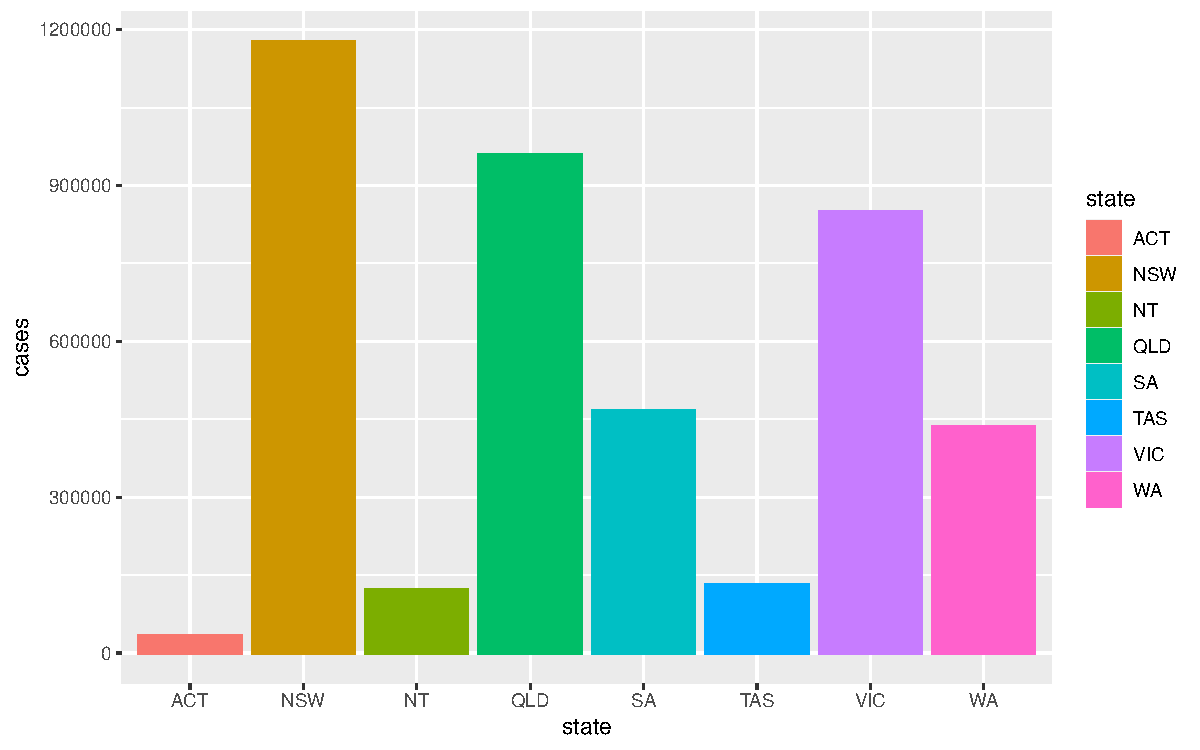
\includegraphics{ETC5513-Assignment4_files/figure-latex/graph1-1.pdf}
\caption{\label{fig:graph1}state-crime}
\end{figure}

The figure above demonstrates high crime cases recorded by NSW, QLD, SA, VIC and WA. However, the high number of crime cases recorded in these states may due to its high population compared to other states/territories like ACT, NT and TAS.

Next, We'd like to look into the frequency of the principal offence in 2018 for top 4 crime-level states. (NSW, QLD, SA and VIC)

\begin{figure}
\centering
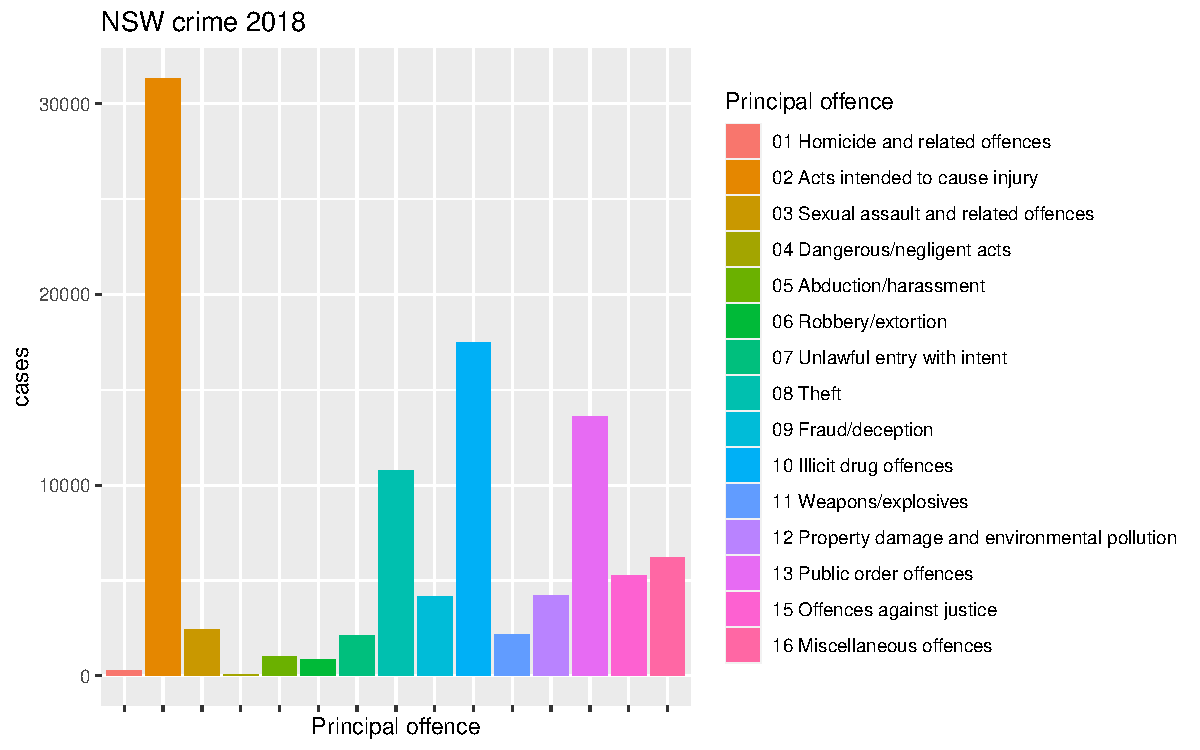
\includegraphics{ETC5513-Assignment4_files/figure-latex/nsw-1.pdf}
\caption{\label{fig:nsw}NSW crime 2018}
\end{figure}

The figure \ref{fig:nsw} demonstrates that 02 Acts intended to cause injury takes the largest proportion in NSW's 2018 crime statistics.

\begin{figure}
\centering
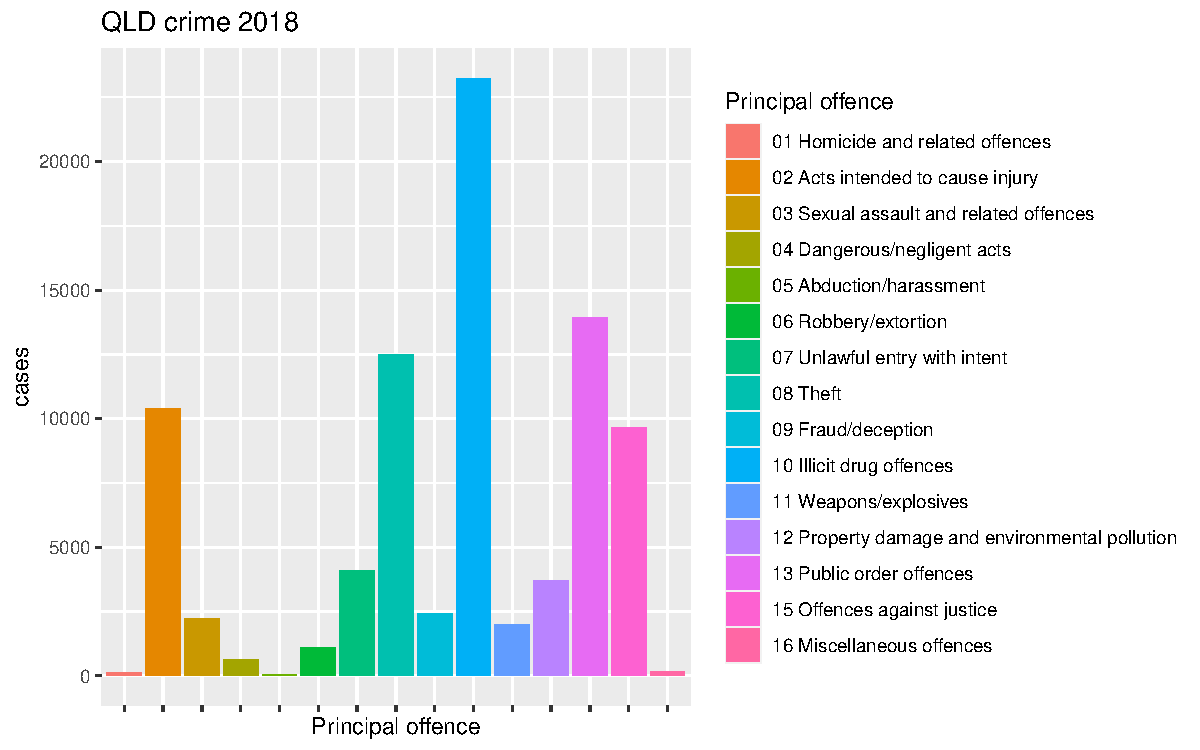
\includegraphics{ETC5513-Assignment4_files/figure-latex/qld-1.pdf}
\caption{\label{fig:qld}QLD crime 2018}
\end{figure}

The figure \ref{fig:qld} demonstrates that 10 Illicit drug offences takes the largest proportion in QLD's 2018 crime statistics. So why some states like QLD have drug offences on rife? Tony Fleming explains in the brisbane times that, ``Largely it is because the Valley and CBD is a night and party precinct. A lot of the drug use is associated with people socialising and whatnot.''\emph{(\textcite{brisbanetimes2019})}

\begin{figure}
\centering
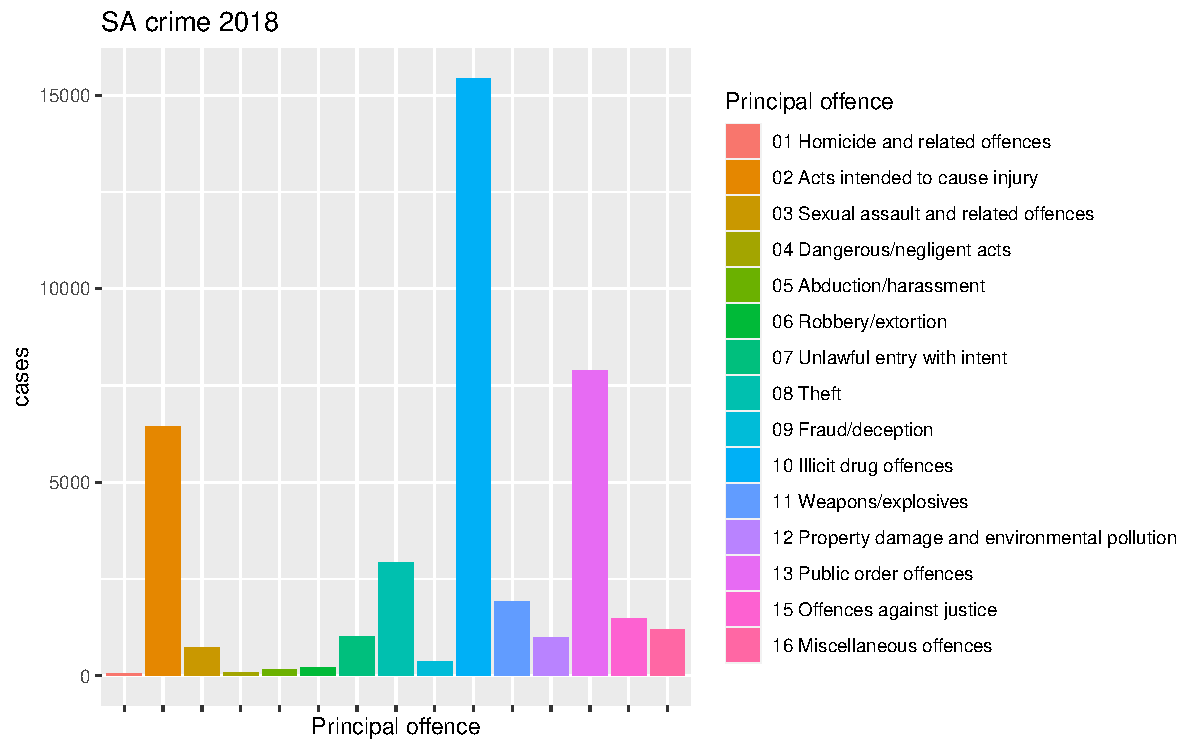
\includegraphics{ETC5513-Assignment4_files/figure-latex/sa-1.pdf}
\caption{\label{fig:sa}SA crime 2018}
\end{figure}

The figure \ref{fig:sa} also represents the outstanding proportion of 10 Illicit drug offences in South Australia's 2018 crime statistics.

\begin{figure}
\centering
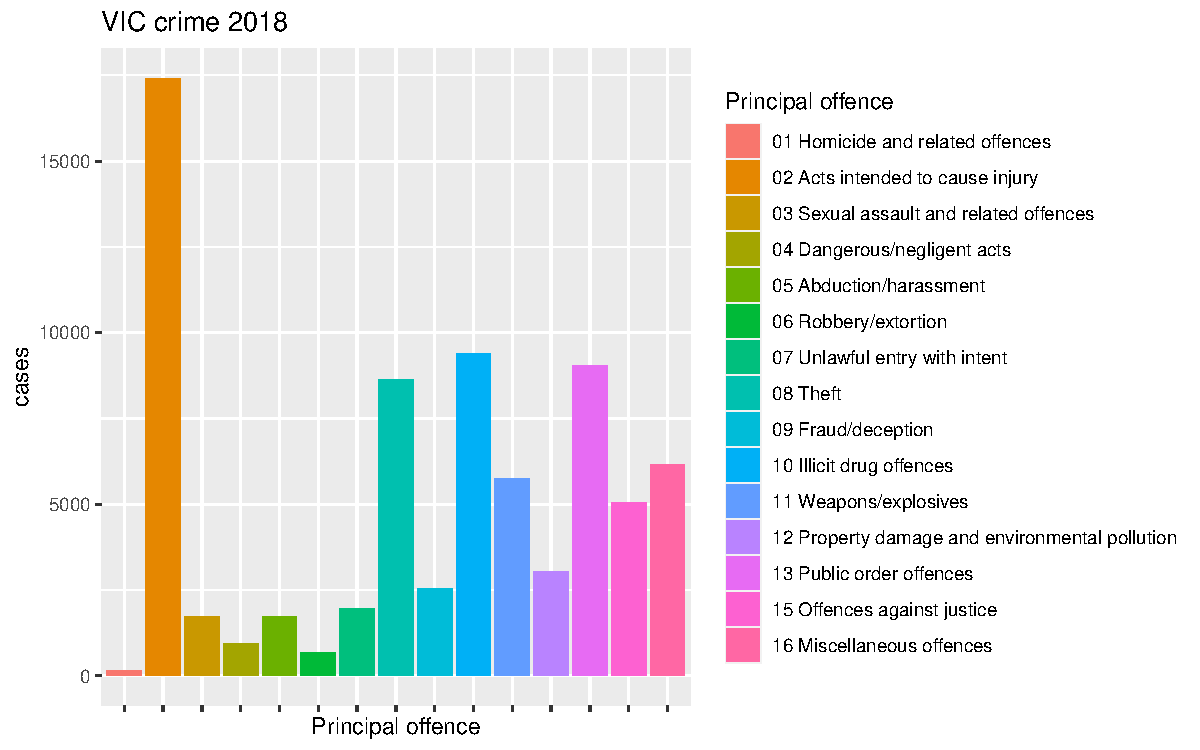
\includegraphics{ETC5513-Assignment4_files/figure-latex/vic-1.pdf}
\caption{\label{fig:vic}VIC crime 2018}
\end{figure}

In the figure \ref{fig:vic}, 02 Acts intended to cause injury resulted in the highest proportion compared to other offences recorded in Victoria's crime statistics.

\begin{table}

\caption{(\#tab:table3.1)Crime statistics 2018 AU}
\centering
\begin{tabular}[t]{l|r}
\hline
State & Proportion\\
\hline
NSW & 27.8823529\\
\hline
VIC & 20.3036936\\
\hline
QLD & 23.6136799\\
\hline
SA & 11.1898769\\
\hline
WA & 10.7370725\\
\hline
TAS & 2.6268126\\
\hline
NT & 2.9699042\\
\hline
ACT & 0.6766074\\
\hline
\end{tabular}
\end{table}

Furthermore, @ref(tab:table3.1) also implies the top 4 states accounted for highest proportion of total crime cases recorded in Australia 2018.

\section*{body 4}

\hypertarget{conclusion}{%
\section{Conclusion}\label{conclusion}}

\printbibliography[title=Reference]

\end{document}

